% \documentclass{article}
% \usepackage[utf8]{inputenc}
% \usepackage{amsmath}
% \usepackage{natbib}
% \usepackage{graphicx}
% \usepackage{astrojournals} % Necesario para nombres de revistas en luis-ref.bib
% \usepackage[spanish, es-minimal]{babel}
% \bibliographystyle{apj}


% \title{Catalog of stationary bowshock arcs in the Orion Nebula}

% \begin{document}
% \maketitle

% \section{Observaciones y descricción de los datos }

\label{chap:theori}

Este capítulo  una descripción de la derivación de los parámetros físicos que gobiernan la naturaleza y estructura de los choques de proa, a partir de las suposiciónes; de que los arcos hiperbólicos y los choques de proa de los proplyds son estacionarios, como una posible consecuencia del equilibrio de presiones; que la cáscara chocada está dominada por la presión térmica y que el flujo de partículas interno y externo que interaccionan para formar los arcos, están dominados por las presiones hidrodinámicas. Se ilustra que en la cáscara chocada se usó la ecuación de estado de los gases ideales para estimar la presión en esta región. Como esta relación está en función de la densidad numérica de partículas, entonces antes de esto construimos una ecuación para la densidad promedio de partículas en función de los parámetros observacionales ya conocidos, esto es en términos del brillo superficial de \ha{} (\(S_{\ha{}}\)), el radio de curvatura (\(R_{c}\)) y el espesor (\(h\)) de la cáscara chocada. Demostramos que no es necesario hacer una corrección de la emisión de ha{} del choque en la emisión de ha{} de la cáscara, puesto que encontramos que el cociente de luminosidad bolométrico entre el choque y la cáscara es muy pequeña, permitiéndonos argumentar que la emisión del choque es despreciable a la emisión de \ha{} y además mostramos que las cáscaras de nuestros objetos están en equilibrio térmico. Hemos encontrado que el cociente entre la longitud de la zona de enfriamiento y la anchura del choque es muy pequeña (\(d_{\text{cool}} \ll h\)).  \\ 

Presentamos el modelo de interacción de dos vientos. Se argumenta que suponemos un modelo en la que que tenemos dos vientos con velocidades constantes, que al colisionar forman una cáscara constituida por dos arcos radiativos.  Ahora  en las regiones externas e internas al choque se usó la presión ram y la ecuación general de la tasa de pérdida de masa para escribir las  presiones de los vientos internos y externos del choque en términos de la tasa de perdida de masa (\(\dot{M}\)), la velocidad del viento \(v\) y las distancias caracteristica (\(D\) y \(R_{0}\)). En el caso del viento interno esto nos permitió  usando el equilibrio de presiones (viene de la suposición de que los choques son estacionarios) escribir los producto  \(\dot{M}_{w}V_{w}\) y \(\dot{M}V\) (flujos de momento) del flujo interno y externo en términos de la presión térmica.\\

Y por último hacemos una  exposición de los resultados astrofísicos. Se muestran los resultados de las estimaciones realizadas de la densidad en la cáscara chocada, la presion en la cáscara,  y el flujo momento interno y externo de los flujos de los objetos de nuestro catálogo, usando los ecuaciones derivadas en la primera parte del capítulo, junto con los parámetros observacionales medidos previamente directo de las observaciones, nos referimos aqui, al brillo superficial de \ha{}  \(S(\ha{})\), los radios de curvatura \(R_{c}\), radio de los choques a lo largo del eje simetría del arco \(R_{0}\) y la anchura de la cáscara \(h\), puesto que estos parámetros son variables de las ecuaciones derivadas teóricamente. donde hemos encontrado que los objetos ubicados en el interior de la nebulosa están confinados por el flujo de momento externo  del viento estelar de las estrellas masivas del Trapecio, mientras que los objetos más distantes requieren un flujo de momento mayor para ser confinados. También ilustramos que el flujo de momento interno no depende de la distancia para los proplyds en el interior de la nebulosa, mientras que el flujo de momento interno de las fuentes más distantes en el que la mitad son proplyds es más pequeño, aunque para los objeto que no son proplyds a estas distancias presentan valores mayores de este parámetro. 

\section{Derivación de parámetros físicos en la cáscara}
\label{sec:phy}

\subsection{Densidad  en la cáscara chocada }
\label{sec:densinty}

Un parámetro físico importante para estudiar la naturaleza de los choques de proa, es la densidad electrónica, así que un primer paso en esta tarea consiste en determinar la densidad promedio de partículas en la cáscara chocada. No obstante existen dos técnicas para estimar esta cantidad física. Una primera técnica consiste en medir la densidad promedio de electrones a través de las observaciones de los efectos de la desexcitación colisional. Esto puede hacerse comparando las intensidades de dos líneas emitidas por un mismo ión desde niveles con energía de excitación similares, así que las tasas de excitación relativas de los dos niveles dependen únicamente del cociente de sus fuerzas de colisión. Si los niveles tienen diferentes probabilidades de transición o diferentes tasas de desexcitación colisional, entonces la población relativa de los dos niveles dpenderá de la densidad, y por consiguiente el cociente de las intensidades de las líneas emitidas también dependerán de la densidad. Los mejores ejemplos de cociente de líneas usados para determinar la densidad electrónica en el rango del óptico son \(\oii~\lambda 3729/\lambda 3726\) y \(\sii~\lambda 6716/\lambda 6731\) \citep{Osterbrock:1989}.\\

La segunda técnica para estimar la densidad electrónica promedio en la cáscara de los choques de proa consiste en usar el brillo superficial de \ha{}, \(S(\ha{})\), obtenido a partir de las observaciones (más adelante daremos más detalles de este método). \citet{Henney:2013a} estimó la densidad electrónica para la cáscara de LL1, usando los dos métodos, es decir empleó el conciente de líneas de \sii{}~\(\lambda 6716/\lambda 6731\) para calcular la densidad en esta zona , y separadamente usó el brillo superficial de \ha{} para el mismo fin, posteriormente comparando los dos resultados encontró que las densidades derivada a partir de los dos métodos fueron muy compatibles. Por tanto para este trabajo hemos utilizado la segunda técnica para estimar la densidad, puesto que contamos con el brillo superficial de \ha{} de la cáscara de todos los arcos de proa de nuestro catálogo, entonces a continuación presentamos una análisis detallado de como determinar la densidad electrónica a partir del brillo superficial de \ha{}, pero antes es importante a hablar un poco sobre la naturaleza de la línea de recombinación de Balmer-\ha{}, debido a que a partir de la emisión de esta línea de recombinación medimos \(S(\ha{})\).    

\subsubsection{Líneas de recombinación de \ha{}}
\label{sec:lines-ha}

La serie de Balmer es un conjunto de líneas espectrales del átomo de hidrógeno que a diferencia de otras líneas de emisión del mismo, las transiciónes ocurren desde los niveles de energía \(n= 3,4,5,...\) al nivel \(n=2\) con \(n\) el número cuántico principal, así cada una de estas transiciones corresponde a una longitud de onda partícular (\(\lambda_{32}\) = 6562.82~\A~(\ha{}; rojo), \(\lambda_{42} = 4861.36~\A{}\) (\(\mathrm{H}\beta\); turquesa), \(\lambda_{52} = 4340.50~\A{}\) (\(\mathrm{H}\gamma\); azul) y \(\lambda_{62} = 4101.77~\A{}\) (\(\mathrm{H}\delta\); violeta)) estas longitudes de onda se han determinado a partir de datos experimentales, además éstas longitudes de onda \(\lambda\) caen dentro de la región visible del espectro electromagnético \citep{Carroll:1996}). Por otro lado, para las líneas de recombinación del átomo de hidrógeno tenemos que la energía de los fotones que se emiten durante las transiciónes está dada por,

\begin{equation}
  \label{eq:energy}
  E = \frac{hc}{\lambda}. 
\end{equation}
 
Según el tratado de Bohr la energía en un estado cuántico es

\begin{equation}
  \label{eq:quantum}
  E_{n} = -13.6~\text{eV}~\frac{1}{n^{2}},
\end{equation}

esta última expresión también nos proporciona la energía del fotón emitido, es decir

\begin{equation}
  \label{eq:energy-}
 E = 13.6~\text{eV}~\left(\frac{1}{n_{\text{Inf}}^{2}}-\frac{1}{n_{\text{Sup}}^{2}}\right).
\end{equation}

 Donde esta es la energía liberada cuando el electrón decae de un nivel de energía, \(n_{\text{Sup}}\), a un nivel de menor energía, \(n_{\text{Inf}}\). No obstante, estos niveles de energía \(n\) constan de diferentes subniveles denotados por el número cuántico \(l\) que tienen ligeramente distintas energías, este fenómeno se le conoce como estructura fina, pero el desdoblamiento entre estos es menor que el ensachamiento térmico de las líneas. Usando las ecuaciones~\ref{eq:energy} y \ref{eq:energy-} para el caso particular de las líneas de recombinación de \ha{} (donde la transición ocurre del nivel superior de energía \(n=3\) al nivel inferior de energía \(n=2\)) tendremos que: 

\begin{equation}
 \label{eq:values-energy-landa}
  E_{32} = 1.889~\text{eV}  ~~ \text{y} ~~
  \lambda_{32} = 6563~\A{}.
 \end{equation}

\subsubsection{Estimación de la densidad a partir del brillo superfical de \ha{} }
\label{sec:brillo}

Empezemos por escribir la relación de brillo superficial, suponiendo que no hay abosorción y que además está corregida por la absorción del polvo;

\begin{equation}
  \label{eq:brillo}
  S_{\ha{}} = \int \eta_{\ha{}} d\zeta \simeq \eta_{\ha{}} \Delta \zeta
\end{equation}  

\noindent en la que  \(\eta_{\ha{}}\) es la emisividad, cuyas unidades son [\(\mathrm{erg~s^{-1}~cm^{-3}~sr^{-1}}\)] y \(\Delta \zeta\) es el camino de la línea de visión a través de la cáscara (más adelante determinaremos \(\Delta \zeta\)). El primero de estos parámetro está dado por,

  \begin{equation}
    \label{eq:emision-coeficiente}
    \eta_{\ha} = \frac{N(\text{H}^0_{n=3})A_{32}}{4 \pi} \left(\frac{hc}{\lambda_{32}}\right) 
  \end{equation}

donde \(A_{32}\) es la probabilidad de transición y \(N(\text{H}^0_{n=3})\) es la densidad numérica de átomos neutros en el nivel \(n=3\). Por otro lado la tasa de recombinaciones por volumen que producen \ha{} es 
\begin{equation}
  \label{eq:recombinaciones}
  \alpha_{\ha} N_{e}N_{\text{H}^{+}}=N(\text{H}^0_{n=3})A_{32}
\end{equation}

donde  \(\alpha_{\ha}\), \(N_{e}\) y \(N_{\text{H}^{+}}\)  son el coeficiente de recombinación efectiva \citep{Osterbrock:2006}, la densidad de electrones y la densidad de núcleos de hidrógeno. La anterior expresión la usamos para introducir el coeficiente de recombinación efectiva en nuestras ecuaciones, puesto que para nuestro estudio es muy conveniente, este coeficiente expresa la probabilidad de que un electrón en el estado \(n=3\) decaiga en cascada hasta el nivel de menor energía \(n=2\). Es importante añadir que cálculos completos de equilibrio estadístico de las cascadas de recombinación han mostrado que el coeficiente de recombinación efectiva depende principalmente de la temperatura electrónica \(T_{e}\), estrictamente hablando es aproximadamente proporcional a la inversa de la  \(T_{e}\) \citep{Pequignot:1991, Nussbaumer:1984} y en menor medida depende de la densidad. También depende de si la serie de Lyman es ópticamente gruesa o delgada, pero en este contexto el relevante es el primer caso, denominado caso B, para la cual las líneas de Lyman son ópticamente gruesas \citep{Hummer:1987}. Hemos supuesto una temperatura electrónica constante de \(\sim 9000~\K \) esto lo justificaremos depués. Para esta temperatura el coeficiente de recombinación efectiva es \(\alpha_{\ha}=1.27\times 10^{-13}\cm^{3}~\text{s}^{-1} \).\\

Por otro lado, al sustituir la Ec. \ref{eq:recombinaciones} en la Ec.~\ref{eq:emision-coeficiente} y teniendo en cuenta que \(N_{e}\simeq N_{\text{H}^{+}} \simeq N_{\text{H}}\) obtenemos que

\begin{equation}
 \eta_{\ha} =  \frac{\alpha_{\ha}N_{\text{H}}^{2}}{4\pi} \left(\frac{hc}{\lambda_{32}}\right)  
\end{equation}

 usando la Ec. (\ref{eq:brillo}) se concluye que,

\begin{equation}
  \label{eq:densidad}
  N_{\text{H}}^{2}=\frac{4 \pi S_{\ha}}{\alpha_{\ha} E_{32} \Delta \zeta}
\end{equation}

\noindent esta expresión representa la densidad promedio de núcleos de hidrógeno en la cáscara, donde \( E_{32} = hc/\lambda_{32}\) es la energía de los fotones de \ha{} y cuyo valor es perceptible en la expresión~\ref{eq:values-energy-landa}. 


\subsection{Proyección en el plano del cielo}
\label{sec:pro}

Otra cosa que debemos  tener en cuenta en relación a los distancias y radios medidios a partir de las observaciones, es que vemos a los choques de proa proyectados en el plano del cielo, es decir que el marco de referencia del observador está rotado un ángulo \(i\) con respecto al marco de referencia del choque. Entonces tendremos que las distancias (\(D\)), y los  radios característicos (\(R_{0}\) y \(R_{c}\)) medidos en la sección anterior no son estimaciones reales de los mismos.\\ 

En este orden de ideas tenemos que las distancias reales son más grandes que las distancias observadas o dicho de otra forma que las distancias proyectadas por un factor de \(1/(\cos i)\). No obstante para una distribución isotrópica el valor mediano de \(|i|\) es \(30^{\circ}\) el cual corresponde a un factor de \(\sim1.155\), esto implica que para este caso la distancia real es mayor \(\sim1.155\) veces que la distancia proyectada.\\ 

Para los radios \(R_{0}\) y \(R_{c}\) el efecto de la inclinación es más complicado, debido a que dependen de la forma exacta del arco, esto es si es esferoidal, hiperboidal, etc, por tanto en este trabajo estos efectos los vamos a ignorar.

\subsection{Estimación de la longitud del camino de la línea de visión a través de la cáscara, \(\Delta \zeta\)}
\label{sec:camino}

\begin{figure}
  \centering
  \includegraphics[width=.8\linewidth, clip]{figuras-tesis/geometri-shock.jpg}
  \caption{Geometría de la cáscara chocada. En el que se supone simetría cilíndrica en el plano del cielo (\(x, y\)), la línea de visión va en dirección al eje de las \(z\).}
  \label{fig:geometria}
\end{figure}

Para una cáscara localmente esférica con radio de curvatura \(R_{c}\) y anchura \(h\) que es observado tangencialmente \citeauthor{Henney:2013a}, suponiendo simetría cilíndrica y el eje de simetría en el plano del cielo (\(x, y\))(ver figura~\ref{fig:geometria1}), la longitud máxima de la línea de visión a través de la cáscara es


\begin{equation}
  \label{eq:line-singht}
   \Delta \zeta = 2\sqrt{2R_{c}h -h^{2}}
\end{equation}

 esto es considerando que la geometría de la cáscara en (\(x, z\)) es igual en (\(x, y\)) (ver figura  \ref{fig:geometria}). Para el caso en que \(h \ll R_{c}\) tendremos que,

\begin{equation}
  \label{eq:vision}
  \Delta \zeta = 2(R_{c}h)^{1/2}
\end{equation}

\begin{figure}
  \centering
  \includegraphics[width=.65\linewidth, trim=20 0.98 140 0.5, clip]{figuras-tesis/geometry-shock2.jpg}
  \caption{Geometría de la cáscara en el plano (\(x, z\)), donde su radio de curvatura \(R_{c}\) es igual que en el plano (\(x, y\)).}
  \label{fig:geometria1}
\end{figure}

\subsection{Presión térmica en la cáscara chocada}
\label{sec:pressur-thermal}

En la cáscara chocada la presión dominante es la presión térmica, debido a que la energía cinética del flujo de partículas cargadas proveniente de la estrella central o proplyd se convierte en energía térmica en la zona chocada, entonces en este sentido tendremos que,

\begin{equation}
  \label{eq:presion-cascara}
  P_{\text{Termica}} = 2 N_{\text{H}} k T 
\end{equation}
 
Donde \(N_{\text{H}}\) dada por la Ec. \ref{eq:densidad}, \(k\) la constante de Boltzmann y \(T\) la temperatura en la cáscara chocada.\\

\section{Emisión del choque versus emisión de la cáscara}
\label{sec:emis}

\begin{figure}
  \centering
  \includegraphics[width=.60\linewidth, clip]{figuras-tesis/zona-interaction}
  \caption{Estructura unidimensional de la zona de interacción para LV 1. El flujo se aleja del frente de ionización del proplyd (región sin sombra), pasa a traveś de un choque después de lo cual se enfría (región con sombra clara), luego  retorna a la temperatura de equilibrio fotoionizado (región con sombra oscura). Tomado de \citet{Henney:2002}.}
  \label{fig:cool}
\end{figure}

En esta sección vamos a demostrar que se puede despreciar la emisión de la zona de enfriamiento en la emisión de \ha{}. Vamos a considerar que el gas en la zona chocada de los arcos de emisión están en equilibrio de fotoionización a una temperatura de \(\simeq10^{4}~\K\) \citep{Henney:2002, Henney:2002a}. No obstante, como se dijo en el capítulo~\ref{chap:introduction} inmediatamente detrás de cada uno de los choques que limitan la cáscara chocada la temperatura del gas se elevará por la termalización de la energía cinética pre-choque, pero este exceso de energía termal es radiada resultando en una gran emisión y de esta manera el gas retorna a su estado de equilibrio. En la figura \ref{fig:cool} se pude ver la zona de interacción donde el flujo de partículas tres regiones, esquemáticamente sería algo como (\(\rho_{0}\), \(v_{0}\), \(T_{0}\)) \(\rightarrow\) (\(\rho_{1}\), \(v_{1}\), \(T_{1}\)) \(\rightarrow\) (\(\rho_{2}\), \(v_{2}\), \(T_{2}\)), donde \(\rho\), \(v\) y \(T\) representan en el mismo orden la densidad volumétrica, la velocidad del flujo y la temperatura en las tres regiones de la zona de interacción, es decir en la región 0 donde el flujo se aleja del frente de ionización (región sin sombra), en la región 1 donde el flujo atraviesa el choque y en el cual se enfría (región con sombra clara) y en la región 2 donde el flujo alcanza la temperatura de equilibrio fotoionizado (región con sombra oscura). Aunque este esquema es para un objeto en particular (LV 1) puede servir para ilustrar este proceso en todos los objetos de nuestro catálogo.\\ 

La luminosidad bolométrica que  es la energía cinética que atraviesa el choque se convierte en energía térmica, posteriormente se caliente y se convierte en enegía radiativa, en este orden de ideas tendremos que la luminosidad de enfriamiento es igual a la luminosidad del choque (\(L_{\text{cool}} = L_{\text{shock}}\)) si \(T_{0} \simeq T_{2}\), es decir si existe equilibrio térmico. Es así que la luminosidad bolométrica del choque en unidades de [\(\mathrm{erg~cm^{-2}~s^{-1}}\)] la podemos escribir como,

\begin{equation}
  \label{eq:lumi-shock}
  L_{\text{shock}} = \frac{1}{2} \rho_{0} v^{3}_{0} A
\end{equation}

Donde \(A\) es el área. Por otro la la luminosidad bolométrica en la cáscara en equilibrio está dada por 

\begin{equation}
  \label{eq:equi}
  L_{\text{shell}} = N^{2}_{2} \Lambda(T_{2}) h A
\end{equation}

Donde \(\Lambda_{2}\) es el coeficiente de enfriamiento del gas en equilibrio en unidades de [\(\mathrm{erg~cm^{3}~s^{-1}}\)] y \(N_{2}\) es la densidad promedio en la cáscara, es decir que es la misma densidad dada por la ecuación \ref{eq:densidad} (\(N_{2} = N_{\text{H}}\)). Ahora que tenemos las expresiónes de las luminosidades para cada zona, las podemos comparar dividiendo una entre la otra considerando que \(N_{2} = M^{2}_{0} N_{0}\) y \(v_{1} = M_{0} c_{0}\) con \(M_{0}\) el número de Mach pre-choque, de esta manera obtenemos para este cociente que

\begin{equation}
  \label{eq:ratio}
  \frac{L_{\text{shock}}}{L_{\text{shell}}} = \frac{0.5 m M_{0} c_{0}^{3}}{N_{2}  \Lambda_{2} h}.
\end{equation}

\begin{figure}
  \centering
  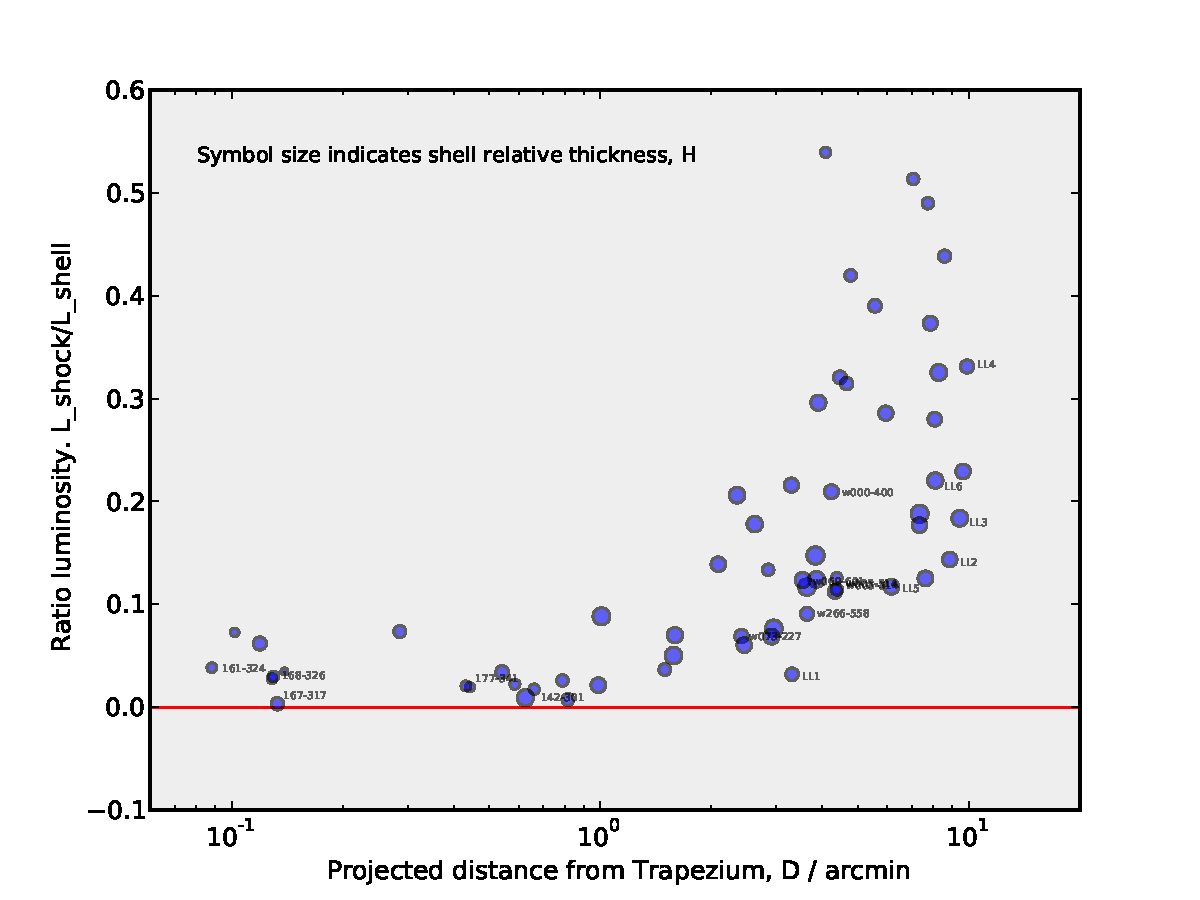
\includegraphics[width=.95\linewidth, clip]{luis-programas/luminosity-ratio}
  \caption{Cociente entre la luminosidad bolométrica del choque \(L_{\text{shock}}\) y la luminosidad bolométrica de la cáscara \(L_{\text{shell}}\) en función de la distancia proyectada desde el Trapecio. El tamaño de los símbolos indican el ancho relativo de la cáscara chocada \(H=h/R_{0}\).}
  \label{fig:ratio-lumi}
\end{figure}

Donde \(m=1.3m_{H}\) es la masa promedio por nucleón y \(c_{0} \simeq \sqrt{kT/m_{H}}\) es la velocidad del sonido fotoionizado. Ahora para un número de Mach \(M_{0} \sim 2.0\), un  coeficiente de enfriamiento de  \(\Lambda_{2} \simeq 3.3\times10^{-24}~\mathrm{erg~cm^{3}~s^{-1}}\) \citep{Osterbrock:2006} y utilizando el ancho de la cáscara y la densidad promedio en la misma la cual es posible determinar a partir de las observaciones usando la Ec. \ref{eq:densidad}, hemos estimado este cociente  de luminosidades bolométricas para nuestros objetos de estudio, los resultados son mostrados en la figura \ref{fig:ratio-lumi}. Pero como lo que nos interesa es la luminosidad de \ha{}, entonces hay que incluir el comportamiento de \(\eta_{\ha{}}/\Lambda\) en función de la temperatura en el cociente determinado previamente, dicho analíticamente sería

\begin{equation}
  \label{eq:ratio-bri}
  \frac{S^{\text{shock}}_{\ha}}{S^{\text{shell}}_{\ha}} = \frac{L_{\text{shock}}}{L_{\text{shell}}} \frac{\eta_{\ha}(T_{1})/\eta_{\ha}(T_{0})}{\Lambda(T_{1})/\Lambda(T_{0})}.
\end{equation}

Ahora, si suponemos que \(\Lambda \propto T^{a}\) y \(\eta_{\ha{}} \propto T^{b}\), tendremos que

\begin{equation}
  \label{eq:ratio-brig1}
   \frac{S^{\text{shock}}_{\ha}}{S^{\text{shell}}_{\ha}} = \left(\frac{T_{1}}{T_{0}}\right)^{b-a} \frac{L_{\text{shock}}}{L_{\text{shell}}}. 
\end{equation}

Aproximadamente los valores de \(a\) y \(b\) son \(a = 2\) y \(b = -1\), es así que \(b - a = -3\). Por otro lado tenemos que 

\begin{equation}
  \label{eq:ratio-tem}
  \frac{T_{1}}{T_{0}} = \frac{1}{16}(5M_{0} - 1)(1 + 3M^{-2}_{0}) \simeq M_{0}
\end{equation}

eso quiere decir que para \(M_{0} = 2.0\) el cociente de temperaturas es \(T_{1}/T_{0} = 2.0\). Esta fracción junto con el valor encontrado para \(b-a\), nos muestra que

\begin{equation*}
  \label{eq:ratio-temp2}
   \left(\frac{T_{1}}{T_{0}}\right)^{b-a} = 0.125 
\end{equation*}

entonces podemos concluir que el cociente de brillo superficial de \ha{} para el choque y la cáscara está dado por

\begin{equation}
  \label{eq:ratio-b}
   \frac{S^{\text{shock}}_{\ha}}{S^{\text{shell}}_{\ha}} = 0.125 \frac{L_{\text{shock}}}{L_{\text{shell}}}
\end{equation}

Con esta última relación aplicada a los resultados mostrados en la figura \ref{fig:ratio-lumi}, podemos decir que el cociente de brillo superficial de \ha{} entre el choque y la cáscara es 0.0 para los objetos situados en las proximidades del Trapecio. Para los objetos LL ubicados a distancia proyectada más grandes la fracción de brillos tiende a aumentar un poco, pero sigue siendo muy pequeña. Entonces podemos concluir que no es necesario hacer una corrección por la emisión de \ha{} del choque, puesto que la contribución de la zona de enfriamiento a la emisión total de \ha{} es despreciable.\\   


Las relaciones de Rankine-Hugoniot dan las condiciones inmediatamnte después del choque. Si \(\rho_{0}\), \(v_{0}\) y \(T_{0}\) es la densidad volumétrica, la temperatura y la velocidad del flujo antes del choque y \(\rho_{1}\), \(v_{1}\) y \(T_{1}\) representan estos mismos parámetros pero a través del choque, entonces el salto de estas cantidades a través del choque estaría dado por (\(\rho_{0}\), \(v_{0}\), \(T_{0}\)) \(\rightarrow\) (\(\rho_{1}\), \(v_{1}\), \(T_{1}\)) para el caso de un choque no radiativo .\\ 

No obstante nos falta comparar la longitud de la zona de enfriamiento \(d_{\text{cool}}\), con la anchura de la cáscara \(h\). Esto lo podemos hacer determinando \(d_{\text{cool}}\) y dividiendo entre \(h\) (valor que determinamos de las observaciones). Para ello hay que considerar que la emisión de la zona de enfriamiento detrás del choque se puede aproximar como la emisión de una capa homogénea con densidad numérica \(N_{1}\), temperatura \(T_{1}\) y una anchura dada por \(d_{\text{cool}} \sim v_{1}t_{\text{cool}}\) donde \(t_{\text{cool}} = 3kT_{1}/(N_{1}\Lambda_{1})\) es el tiempo de enfriamiento y \(v_{1} = M_{1}(T_{1}/T_{0})^{1/2}c_{0}\) es la velocidad pos-choque, en estas dos últimas expresiones \(\Lambda_{1}\) y \(M_{1}\) representan el coeficiente de enfriamiento en la zona de enfriamiento y el número de Mach en la zona pos-choque. O podemos determinar esta fracción utilizando el cociente de la luminosidad bolométrica del choque entre la luminosidad bolométrica de la cáscara, no es una técnica tan exacta para determinar el cociente entre  \(d_{\text{cool}}\) y \(h\) como la descrita anteriormente, pero si nos permite obtener un aproximado de que tan pequeña es la longitud del ancho de la zona de enfriamiento con respecto a la anchura del choque, además este procediminto tiene la ventaja de que ya conocemos la fracción de luminosidades bolométricas, por tanto utilizamos en este trabajo esta última técnica para este fin. En esta sentido tenemos que 

\begin{equation}
  \label{eq:lumi-long}
  \frac{L_{\text{shock}}}{L_{\text{shell}}} = \frac{N^{2}_{1}d_{\text{cool}}\Lambda_{1}}{N^{2}_{2}h\Lambda_{2}}
\end{equation}

como se mencióno arriba que \(\Lambda = T^{a}\) y dado que la cáscara retorna a su temperatura de equilibrio esto es que \(T_{0} = T_{1}\), entonces esta expresion se convierte en,

\begin{equation*}
 \frac{d_{\text{cool}}}{h} = \frac{N^{2}_{2}\Lambda_{0}}{N^{2}_{1}\Lambda_{1}} \frac{L_{\text{shock}}}{L_{\text{shell}}} = \frac{N^{2}_{2}}{N^{2}_{1}}\left(\frac{T_{1}}{T_{0}}\right)^{-a} \frac{L_{\text{shock}}}{L_{\text{shell}}}.
\end{equation*}

Pero también sabemos que \(N_{2}=M^{2}_{0}N_{0}\) y que \(N_{1} = 4N_{0}/(1+3M_{0}^{-2})\) (ver Henney 2002), en esta medida la relación anterior se transforma en  

\begin{equation}
\label{eq:longui}
 \frac{d_{\text{cool}}}{h} = \left(\frac{M^{2}_{0}+3}{4}\right)^{2} \left(\frac{T_{1}}{T_{0}}\right)^{-a} \frac{L_{\text{shock}}}{L_{\text{shell}}}.
\end{equation}

Previamente dijimos que \(a = 2\), con lo cual obtenemos que \((T_{1}/T_{0})^{-2} \simeq 0.3\) y como hemos considerado un valor para el número de Mach de \(M_{0}\sim 2.0\), entonces estas premisas apicadas a la ecuación \ref{eq:longui} nos muestra que el cociente entre \(d_{\text{cool}}\) y \(h\) es del mismo orden que el cociente entre \(L_{\text{shock}}\) y \(L_{\text{shell}}\) (\(d_{\text{cool}}/h \sim L_{\text{shock}}/L_{\text{shell}}\)), es decir que en los objetos más próximos al Trapecio el cociente \(d_{\text{cool}} / h\) es aropximadamente 0.0, pero  puede llegar a un valor de 0.5 para los arcos más lejanos, como ocurre en el cociente de luminosidades bolométricas entre el choque y la cáscara (ver figura \ref{fig:ratio-lumi}), por tanto podemos argumentar que \(d_{\text{cool}} \ll h\). Esto significa que la cáscara chocada está en equilibrio térmico, es decir se puede establecer un salto directo desde la zona antes del choque a la cáscara chocada, es decir (\(\rho_{0}\), \(v_{0}\), \(T_{0}\)) \(\rightarrow\) (\(\rho_{2}\), \(v_{2}\), \(T_{2}\)) donde el subíndice 2 indica que se trata de la cáscara chocada, que como ya se ha dicho está en equilibrio térmico porque se cumple la condición de que \(T_{0} = T_{2} = T = 10^{4}~\K\). Se trata de la misma temperatura de la ecuación \ref{eq:presion-cascara}. \\  

\section{Interacción de dos vientos}
\label{sec:interaction}

Consideramos un modelo de interacción de dos vientos porque en este modelo se hace la suposición de que dos vientos con cierta velocidad colisionan y durante este proceso forman una cáscara limitada por dos contornos bien definidos, como se puede ver en las observaciones tratadas en esta tesis, dicho de otra manera, forman una cáscara constituida por dos choques radiativos. Con esta cualidad de los bordes (están bien definidos) se puede establecer una geometría aproximada de la cáscara, de donde se pueden extraer parámetros útiles para estudiar la naturaleza de la cáscara y de los flujos que intervien para formarla. Entonces la geometría de este modelo está caracterizada por las variables \(D,~R_{0}\), \(R\) y \(h\), los cuales representan en el mismo orden; la distancia de la fuente a \thC{}, los radios desde el arco de proa a la estrella central a lo largo del eje del choque, el radio de curvatura de la cáscara en su eje de simetría y la anchura de la cáscara. Este radio de curvatura, \(R_{c}\), no es necesariamente igual al radio de curvatura empírico medido de las observaciones, porque este último hace referencia al radio proyectado del círculo fijado a los puntos donde se encuentran los choques de proa en las observaciones, mientras que el radio de curvatura teórico hace referencia al radio de los círculos en el eje de simetría de la cáscara chocada (ver figura \ref{fig:geometria}). Como ya se ha reiterado, las suposiciones para este tipo de modelo son las siguientes:
\begin{enumerate}
\item Las cáscaras chocadas están en estado estacionario (tiempo dinámico \(\ll\) tiempo evolutivo), puesto que no se les han detectado movimientos propios. Esto puede ser el resultado del equilibrio de presiones en estas regiones.
\item La aceleración debido a la gravedad u otras fuerzas como por ejemplo de la radiación, es despreciables.
\item En los vientos (viento estelar o el flujo fotoevaporado según sea el caso) domina la presión hidrodinámica y en la cáscara chocada domina la presión térmica (ver figura~\ref{fig:interaction}).  
\end{enumerate}

\begin{figure}
  \centering
  \includegraphics[width=.95\linewidth, clip]{figuras-tesis/pressures-bowshocks.jpg}
  \caption{Choque formado por la interacción de dos flujos. El viento en el ambiente está dominado por la presión hidrodinámica  (\(P_{\text{Hyd}}(\Out{})\)), al igual que el viento generado por la estrella T-Tauri o el proplyd, esto es, (\(P_{\text{Hyd}}(\In{})\)). Por otro lado la cáscara chocada está dominada por la presión térmica (\(P_{\text{Termica}}\)).}
  \label{fig:interaction}
\end{figure}
 
Con estas suposiciones es posible determinar el flujo de momento del viento interno, usando la presión en la cáscara estimada en la sección anterior y la presión ram que a continuación estimaremos.  

\subsection{Presión hidrodinámica}
\label{sec:pressure}

 En términos generales la tasa de pérdida de masa está dada por

\begin{equation}
  \label{eq:perdida-masa}
  \dot{M}=4\pi \rho v R^{2}
\end{equation}

Donde \(\mathrm{\rho}\), \(v\) y \(R\) son la densidad del flujo, la velocidad del flujo y la distancia a la fuente en el mismo orden. Por otro lado la presión del viento estelar es,

\begin{equation}
  \label{eq:presion-viento}
  P=\rho v^{2}
\end{equation}

si combinamos las ecuaciones \ref{eq:perdida-masa} y \ref{eq:presion-viento} obtenemos,

\begin{equation}
  \label{eq:presin-interna}
  P=\frac{\dot{M} v}{4 \pi R^{2}}. 
\end{equation}
 
En general esta (Eq.~\ref{eq:presin-interna}) es la presión ram ejercida por un flujo de partículas, en términos de \(\dot{M}\) y \(v\). Particularmente para nuestro modelo tendremos  dos tipos de presiones hidrodinámicas; una corresponde a la presión generada por el viento estelar proveniente del Trapecio dada por

\begin{equation}
  \label{eq:presion-externa}
   P_{\text{Hyd}}(\Out{})=\frac{\dot{M}v}{4 \pi D^{2}}
\end{equation}

donde \(D\) es la distancia de la fuente a \thC{}, \(\dot{M}\) es la tasa de pérdida de masa de la estrella masiva del Trapecio y \(v\) es la velocidad del viento estelar externo. Y otra que corresponde a la presión ejercida por el viento de la estrella T-Tauri o proplyd

 
\begin{equation}
  \label{eq:presion-interna}
  P_{\text{Hyd}}(\In{})=\frac{\dot{M}_{w} V_{w}}{4 \pi R_{0}^{2}}.
\end{equation}

Las variables de la ecuación anterior se refieren a la tasa de pérdida de masa y la velocidad del viento de la estrella T-Tauri, además de esto \(R_{0}\) representa la distancia de la estrella o proplyd al choque.

\subsection{Flujo de momento  del viento externo  y del viento interno }
\label{sec:momento}

De acuerdo a la suposición 1, existe un equilibrio de presiones tal que;
 
\begin{equation}
  \label{eq:igualda-presion}
  P_{\text{Hyd}}(\Out{})=P_{\text{Termica}}=P_{\text{Hyd}}(\In{}).
\end{equation}

Ahora si sustituimos la Ec. \ref{eq:presion-externa} en la anterior expresión y luego hacemos los mismo con la Ec.~\ref{eq:presin-interna}, podemos escribir el flujo de moneto interno y separadamnete el externo en términos de la presión térmica. 

\begin{equation}
  \label{eq:momentum-out}
   \dot{M}V = 4 \pi  D^{2}  P_{\text{Termica}}. 
\end{equation}


\begin{equation}
  \label{eq:momentum}
   \dot{M}_{w}V_{w} = 4 \pi  R_{0}^{2}  P_{\text{Termica}}. 
\end{equation}

Donde \(P_{\text{Termica}}\) está dada por la ec~\ref{eq:presion-cascara}. 

\section{Resultados físicos: cálculo de las propiedades físicas }
\label{sec:results}

\begin{figure}
  \centering
   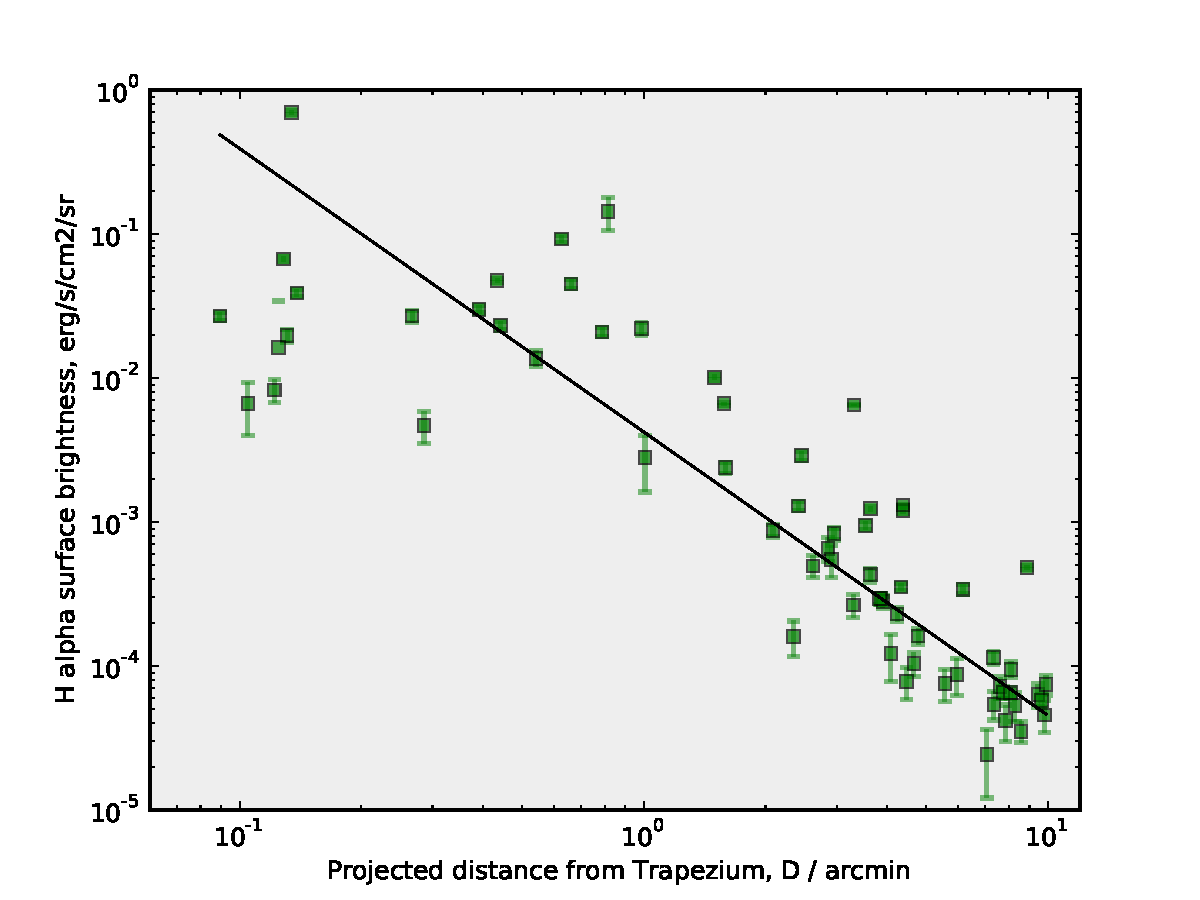
\includegraphics[width=.95\linewidth, clip]{luis-programas/brightness-shell_acs_Vs-D_new.pdf}
  \caption{Brillo superficial de \ha{}  corregido por extinción y por la emisión de \nii{}, obtenido a partir de las imágenes de \citeauthor{Bally:2006a} en función de la distancia proyectada desde Trapecio. La línea respresenta un ajuste líneal dada por \(S(\ha{})\sim D^{-1.97}\).} 
  \label{fig:bright}
\end{figure}


Para empezar hemos determinado el brillo superficial de \(\ha{}~\lambda6563\) usando las imágenes de Bally (cámara ACS-F658N) para posteriormente determinar otros parámetros físicos como la densidad numérica de partículas en la cáscara, como veremos más adelante. Para nuestros propósitos hemos determinado el brillo superficial de \ha{} a partir de las imágenes de Bally. Como ya sabemos estas observaciones se basan en líneas de emisión de \ha{} contaminadas por las líneas de \nii{}, es así que el brillo medido que  mostramos en la figua~\ref{fig:bright} es el resultado de haber hecho la correción por la emisión de \nii{}  y en el mismo orden de ideas a este resultado de las estimaciones del brillo se le suma la correción por extinción. En la figura se puede ver que el brillo superficial  de \ha{} cae con la distancia proyectada desde Trapecio, esto es con la relación \(S(\ha{})\sim D^{-1.97}\) (esta relación es obtenida a partir de un ajuste lineal realizado sobre los  puntos graficados), así que tenemos que los objetos en el interior de la nebulosa que entre otras cosas son proplyds conocidos son más brillantes que los que se ecuentran más alejados. 

\subsection{Densidad promedio en la cáscara}
\label{sec:density}

\begin{figure}
  \centering
   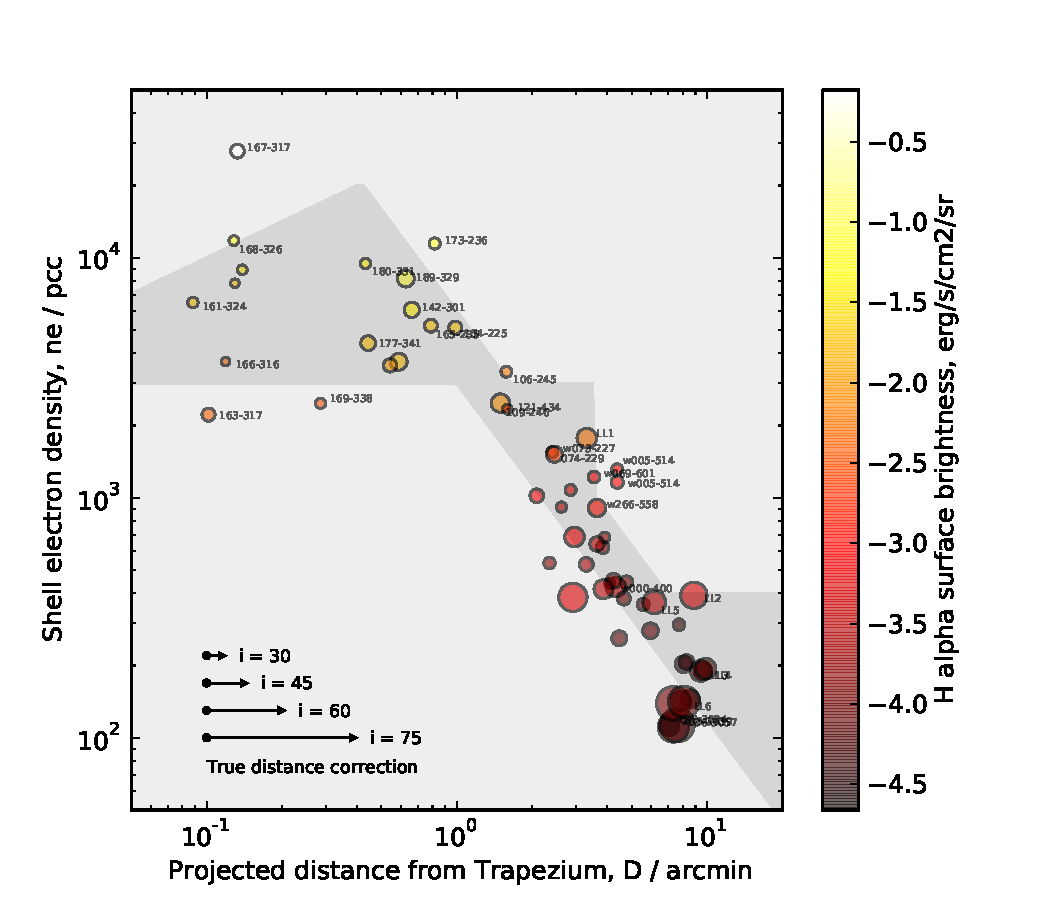
\includegraphics[width=\linewidth, clip]{luis-programas/will-nshell-vs-D.pdf}
  \caption{Densidad electrónica calculada a partir de la ecuación \ref{eq:densidad} en función de la distancia proyectada desde \(\theta^1\ \text{Ori}\ \text{C}\). El tamaño de los puntos indica que tan grande es el camino de visión en la zona chocada si los comparamos entre si. Las flechas en la parte inferior izquierda representan la distancia corregida por la inclinación de la distancia proyectada (observada) de los arcos de emisión con respecto a la verdadera distancia desde \thC{}, para los ángulos de inclinación; \(i = 30^{\circ}, 45^{\circ}, 60^{\circ}, 75^{\circ}\). Por otro lado la escala de colores representa el brillo superficial de \ha{} corregido por extinción y por la emisión de \nii{} en la cáscara chocada en unidades de [\(\mathrm{erg~s^{-1}~cm^{-2}~sr^{-1}}\)]. Por último la franja oscura representa la densidad electrónica del gas ambiental de la nebulosa, el ancho de la franja indica la dispersión del valor de la densidad a cada distancia \citep{Odell:2010, Mesa:2008}.}
  \label{fig:density}
\end{figure}

Dado que a partir de las observaciones hemos podido determinar el brillo superficial de \ha{} realizando un poco de fotometría como se puede apreciar previamente y además como hemos determinado el camino de la línea de visión en la cáscara chocada (\(\Delta\zeta\)), mediante la Ec. \ref{eq:vision}, fue posible para nosotros determinar la densidad promedio de partículas (\(N\)) usando la ecuación \ref{eq:densidad}, específicamente en esta zona (en la cáscara chocada) para los diferentes objetos LL y los proplyds. Hay que subrayar que hemos usado cómo distancia a la Nebulosa de Orión \(436 \pm 20~\text{pc}\) \citep{Odell:2008}, para pasar  de unidades en arcsec a unidades físicas (cm), las unidades de los radios de curvatura \(R_{c}\) y la longitud del ancho de las cáscaras \(h\), esta conversión fue necesaria para calcular la densidad promedio de partículas en la cáscara (ver la sección \ref{sec:phy}).\\

En esta medida, en la figura \ref{fig:density} se logra apreciar que la cáscara chocada de los objetos que están más cerca de las estrellas masivas del Trapecio, presentan una densidad electrónica mayor que los que se encuentran a las afueras de la nebulosa. Esta tendencia de que las densidades sean menores a grandes distancia es congruente con el comportamiento del gas ambiental en la nebulosa. Argumentamos esto porque \citet{Odell:2010} derivaron la densidad del ambiente nebular en las regiones externas de la nebulosa (franja oscura a partir de \(\sim 1.0\) arc de distancia) usando el cociente de líneas de \(\sii~\lambda 6716/\lambda 6731\) y de \(\cliii~\lambda 5518/\lambda 5531\) encontrando que estas caen con la distancia proyectada desde \thC{}. En las regiones internas de la nebulosa y cercanas al Trapecio vemos que la densidad medida por \citet{Mesa:2008} del gas ambiental de la nebulosa (franja oscura en las regiones cercanas  al Trapecio) concuerda con las densidades en las cáscaras chocadas de los arcos de proa medidas por nosotros, apoyando el argumento de que la densidad de las cáscaras es congruente con la densidad del gas nebular.    

\subsection{Flujo de momento externo: \(\dot{M}\text{V}\) }
\label{sec:pressure}

\begin{figure}
  \centering
  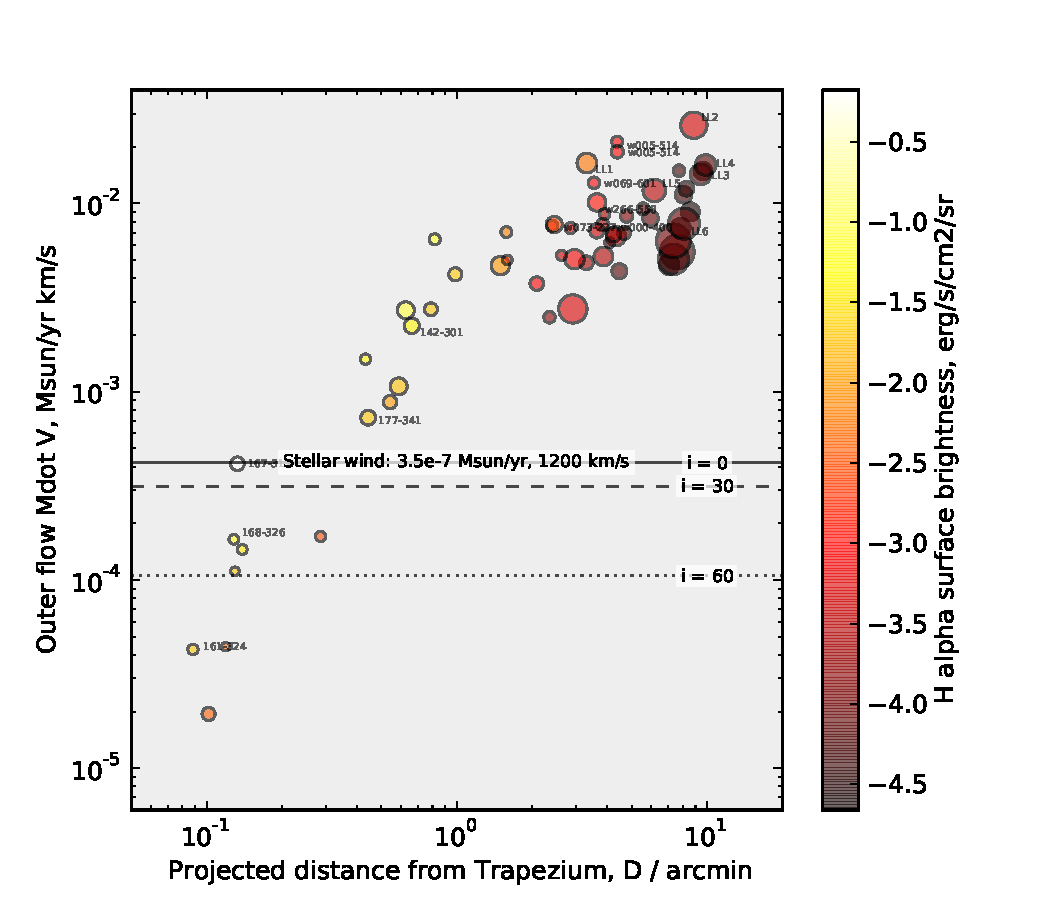
\includegraphics[width=\linewidth, clip]{luis-programas/will-MdotVout-vs-D.pdf}
  \caption{Flujo de momento del viento externo en función de la distancia proyectada desde \thC{}. Lo símbolos de colores representan el flujo de momento externo de cada objeto de nuestro catálogo estimado a partir de la ecuación \ref{eq:momentum-out} y suponiendo que es un flujo esférico proveniente del núcleo de la nebulosa. La línea continua representa el flujo de momento del viento estelar  suponiendo que no hay inclinación, esto es para \(i = 0^{\circ}\), la línea discontinua representa el mismo flujo de momento externo del viento estelar para una distancia proyectada cuando se cambia el ángulo de inclinación desde la distancia (\(i = 0^{\circ}\)), esto es para un ángulo de inclinación de \(i = 30^{\circ}\) y la línea de puntos también representa el flujo de momento externo para una distancia proyectada con un ángulo de inclinación de \(i = 60^{\circ}\). La escala de colores indica el brillo superficial de \ha{}.}
 \label{fig:pressure}
\end{figure}

Usando la ecuación \ref{eq:momentum-out} de \S\ref{sec:momento} se estimó el flujo de momento externo, suponiendo que es un flujo esférico que proviene del centro de la nebulosa. Para ello en primera instancia determinamos la presión térmica en la cáscara chocada a partir de la densidad electrónica calculada en \S\ref{sec:density} y utilizando una temperatura para la cáscara en equilibrio de \(10^{4}~\K\) como hemos demostrado previamente. Por otro lado determinamos el flujo momento externo del viento estelar hipersónico de la estrella másiva \thC{} del Trapecio, usando una tasa de pérdida de masa de \(\dot{M} = 3.5 \times 10^{-7}~\msolagno\) y una velocidad de \(v = 1200~\mathrm{km~s^{-1}}\) para este viento estelar. \\

Ahora bien, la figura \ref{fig:pressure} es el resultado de tales estimaciones. En ella estamos comparando los flujos de momento externo de los objetos LL y de los proplyds (símbolos de colores en la gráfica), con el flujo de momento generada por el viento estelar (líneas continuas  y discontinuas  de color  negro en la gráfica). Se observa que flujo de momento es mayor en los objetos más distantes del Trapecio que los proplyds que se encuentran en el interior de la nebulosa, además se puede ver que el flujo de momento de los arcos interiores de la nebulosa coincide con el flujo de momento del viento de la estrella masiva, indicando que los choques de los proplyds en el interior están confinados por el hipersónico viento estelar. Lo contrario sucede con los arcos hiperbólicos LL más distantes del Trapecio, puesto que a partir de 0.05~pc empieza a haber una discrepancia muy marcada entre los dos flujos de momento, indicando que estos objetos no están interactuando con el viento estelar.  

\subsection{Flujo de momento interno: \(\dot{M}_{w}\text{V}_{w}\) }
\label{sec:momentum}

\begin{figure}
  \centering
  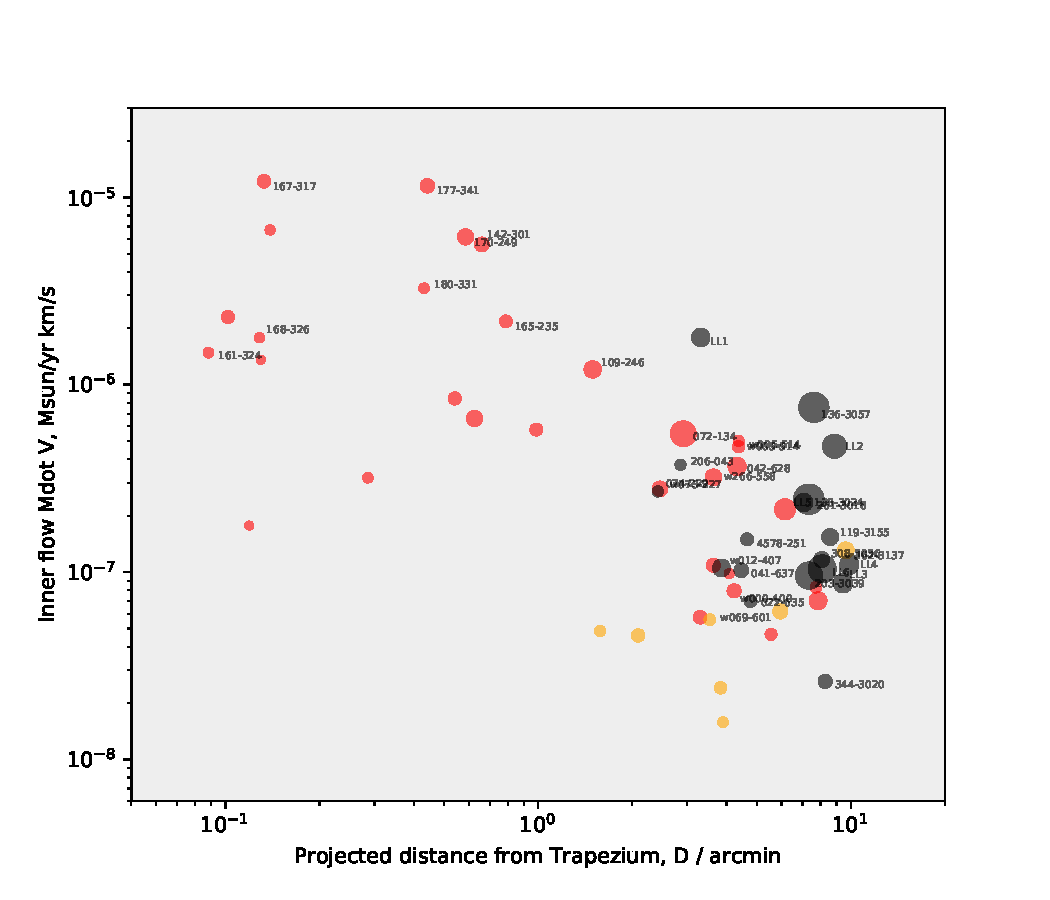
\includegraphics[width=\linewidth, clip]{luis-programas/will-MdotV-vs-D.pdf}
  \caption{Flujo de momento interno  en función de la distancia proyectada. El color de los símbolos indican: Rojo; son verdaderos proplyds, naranja; podrían tratarse de proplyds, negro; no son proplyds. El tomaño de los símbolos representan el tamaño de la línea de visión (\(\Delta\zeta\)) en la cáscara chocada.  }
 \label{fig:flow}
\end{figure}


Hemos determinado el flujo de momento interno para los objetos de nuestro catálogo a partir de las presiones de estancamiento, presiones con las cuales se obtuvo la ecuación \ref{eq:momentum}, con esta ecuación fue posible determinar el ya mencionado flujo de momento interno, en este orden de ideas se utilizaron los valores de la presión térmica determinados arriba, junto con los valores de los radios \(R_{0}\) internos de los choques LL para este fin. Asi que en la figura \ref{fig:flow} se ilustran dichos resultados.\\

No obstante, en la figura~\ref{fig:flow} se logra apreciar que para los objetos clasificados como proplyds en nuestro catálogo (símbolos de color rojo) y que están dentro de la distancia de \(0.2\)~pc del Trapecio muestran grandes flujo de momento interno y que este flujo no varía con la distancia proyectada. Ahora bien, en los proplyds y supuestos proplyds (símbolos de color naranja), se observa una caida del parámetro \(\dot{M}_{w}V_{w}\) (flujo de momento interno) a partir de \(0.2\)~pc, además se puede ver que en estos arcos el flujo de momento es más débil que los arcos interiores. Esto es evidencia de que la tasa de pérdida de masa de los proplyds cae con la distancia, debido probablemente  a que el flujo de fotones FUV (ultravioletas lejano), responsables directo de la destrucción inevitable de los discos de acreción, decrecen con la distancia a la estrella masiva \thC{}. Por último, para el caso de los objetos que no son proplyds (símblos de color negro) situados en las regiones externas de la nebulosa, se observa que tienden a tener  flujos de momentos interno mayores que los proplyds ubicados a las mismas distancias, unos argumentos que pueden explicar estás grandes pérdidas de masa en estos objetos son; que puede haber un efecto de fotoevaporación interna por el efecto de los rayos x cromosféricos que se originan en la estrella central y que además estás estrellas tienden a ser de las más brillantes \citep{Clarke:2014}.\\ 


%\bibliography{luis-ref}

%\end{document}
